% --------------------------------------------------------------------------
% Template for IWAENC 2022 papers; to be used with:
%          spconfa4.sty  - ICASSP/ICIP LaTeX style file, and
%          IEEEbib.bst - IEEE bibliography style file.
%
% (Last modified by H. Loellmann, LMS, FAU Erlangen-Nuremberg, Jan. 2020)
%
% --------------------------------------------------------------------------

\documentclass{article}
\usepackage[preprint]{spconfa4}
\usepackage{amsmath,graphicx}
\usepackage[dvipsnames]{xcolor}
\usepackage{tikz}
\usetikzlibrary{arrows,snakes,backgrounds,matrix,patterns,positioning,fadings}
\usepackage{standalone}
\usepackage{subfig}
\usepackage{upgreek}
\usepackage{nicefrac}
\usepackage{dsfont}
\usepackage{bm}
\usepackage{cancel}
\usepackage{amsbsy}
\usepackage{algorithm}
\usepackage{algpseudocode}
\usepackage{lipsum}
\usepackage{harpoon}
\usepackage{comment}
\newenvironment{note}
 {\par\textcolor{Blue}{\bfseries Note:} \color{Blue}\ignorespaces}
 {\par}
\newenvironment{attention}
 {\par\textcolor{red}{\bfseries Attention:} \color{red}\ignorespaces}
 {\par}
\usepackage{hyperref}
\hypersetup{
	colorlinks,
	linkcolor={blue!80!black},
	citecolor={blue!80!black},
	urlcolor={blue!80!black}
}

\newcommand{\mtxb}[1]{\bm{\mathrm{#1}}}
\newcommand{\T}{{\mathrm{T}}}
\newcommand{\herm}{{\mathrm{H}}}
\newcommand{\ev}[1]{\mathrm{E} \left\lbrace #1 \right\rbrace}

% \excludecomment{note}
% \excludecomment{attention}

% Common variables
\newcommand{\h}{\mtxb{h}}
\newcommand{\x}{\mtxb{x}}
\newcommand{\R}{\mtxb{R}}
\newcommand{\w}{\mtxb{w}}
\newcommand{\z}{\mtxb{z}}
\newcommand{\uu}{\mtxb{u}}
\newcommand{\aRho}{\mtxb{P}}
\newcommand{\hf}{\underline{\bm{h}}}
\newcommand{\xf}{\underline{\bm{x}}}
\newcommand{\Rf}{\bm{\mathcal{R}}}
\newcommand{\wf}{\underline{\bm{w}}}
\newcommand{\zf}{\underline{\bm{z}}}
\newcommand{\uuf}{\underline{\bm{u}}}
\newcommand{\aRhof}{\bm{\mathcal{P}}}
\newcommand{\I}{\mtxb{I}}
\newcommand{\Cset}{\mathcal{C}}
\newcommand{\Csetb}{\bar{\mathcal{C}}}
\newcommand{\Mset}{\mathcal{M}}
\newcommand{\Nset}{\mathcal{N}}



% IMPORTANT: Add copyright notice by uncommenting the appropriate line
%----------------------------------------------------------
% For papers in which all authors are employed by the US government,
% \copyrightnotice{U.S. Government work not protected by U.S. copyright}

% For papers in which all authors are employed by a Crown government (UK, Canada, and Australia)
% \copyrightnotice{978-1-6654-6867-1/22/\$31.00~\copyright2022 Crown}

% For papers in which all authors are employed by the European Union,
% \copyrightnotice{978-1-6654-6867-1/22/\$31.00~\copyright2022 European Union}

% For all other papers the copyright notice is
\copyrightnotice{978-1-6654-6867-1/22/\$31.00~\copyright2022 IEEE}

% Title.
% ------
\title{CROSS-RELATION-BASED FREQUENCY-DOMAIN BLIND SYSTEM IDENTIFICATION USING ONLINE ADMM}
%
% Single address.
% ---------------
\name{Matthias Blochberger\sthanks{This research work was carried out at the ESAT Laboratory of KU Leuven, in the frame of the SOUNDS European Training Network. This project has received funding from the European Union's Horizon 2020 research and innovation programme under the Marie Skłodowska-Curie grant agreement No. 956369.}, Filip Elvander\sthanks{This work was supported in part by the Research Foundation - Flanders (FWO) grant 12ZD622N.}, Randall Ali\(^*\), Toon van Waterschoot\(^*\)}
\address{KU Leuven\\Department of Electrical Engineering (ESAT)\\STADIUS Center for Dynamical Systems, Signal Processing and Data Analytics \\3001 Leuven, Belgium}
%
\begin{document}
%\ninept
%
\maketitle
%
\begin{abstract}
    In this contribution, we propose a cross-relation-based adaptive algorithm for blind identification of single-input multiple-output (SIMO) systems in the frequency domain using the alternating direction method of multipliers (ADMM).
    The proposed algorithm exploits the separability of the cross-channel relations by splitting the multichannel identification problem into lower-dimensional sub-problems with lowered computational complexity and can be solved in parallel.
    Each sub-problem yields estimates for a subset of channel spectra, which then are combined into a consensus estimate per channel using general form consensus ADMM in an adaptive updating scheme.
    With numerical simulations, we show that it is possible to achieve estimation errors and convergence speeds comparable to low cost frequency-domain algorithms.
\end{abstract}
%
\begin{keywords}
    blind system identification, multichannel signal processing, ADMM, Online-ADMM
\end{keywords}
%
\section{Introduction}
\label{sec:intro}
The problem of blind system identification (BSI), also called blind multichannel identification (BMCI), which aims to estimate channel impulse responses of an unknown system from output signals only has been subject of extensive research over the recent decades.
Early methods used higher-order statistics (HOS) \cite{} for channel estimation, however the high complpexity led to research into methods only using second-order statistics (SOS).
The first to be proposed was the cross-relation (CR) method \cite{}, which this contribution focuses on as well.
Other relevant approaches to solve the SIMO BSI problem are subspace methods \cite{}, least-squares approach \cite{} and maximum-likelihood \cite{} methods.

Out of various multichannel BSI algorithms which have been proposed, adaptive least mean squares (LMS) algorithms in time \cite{} and frequency domain \cite{} are the ones most widely used.
The NMCFLMS algorithm is an efficient algorithm utilizing the fast Fourier transform (FFT) which has been extended to include constraints to improve robustness to noise and performance on acoustic impulse responses (RNMCFLMS \cite{}, \(l_p\)-RNMCFLMS \cite{}).

The alternating direction method of multipliers (ADMM) \cite{} solves convex optimization problems by splitting them into smaller sub-problems, each less complex to solve than the original one.
It has found applications in a large number of areas such as machine learning \cite{} or control systems \cite{}.
Here, we use ADMM to separate the inter-channel cross-relations to form smaller sub-problems involving overlapping subsets of the entire channel set and use constraints to find a consensus on the overlapping estimated parameters of the sub-problems.
This reduces the theoretical time effort to find a solution by complexity reduction and additionally enabling parallel processing of sub-problems.
The ADMM update steps solving for the sub-problem estimates, the overall consensus estimate and dual variables, are applied in a block processing scheme forming an adaptive algorithm also referred to as Online-ADMM \cite{}.


% \lipsum[1-4]

% #############################################################################
% #############################################################################
\section{Problem statement}
\label{sec:problem_statement}


% #############################################################################
\subsection{Signal Model}
\label{ssec:signal_model}
We define the acoustic SIMO system with the input signal \(\mtxb{s}(n) = \begin{bmatrix}
    s(n)&s(k-1)&\ldots&s(k-2L+2)
\end{bmatrix}^{\T}\) and \(i \in \Mset\) with \(\Mset \triangleq \{1,\ldots,M\} \) outputs 
\(
    \x_i(n) = \begin{bmatrix}
        x_i(n)&x_i(k-1)&\ldots&x_i(k-L+1)
    \end{bmatrix}^{\T}
\).
Each output \(\x_i\) is the convolution of \(\mtxb{s}\) with the respective channel impulse response \(\h_i\) with additive noise term \(\mtxb{v}_i\), assumed to be zero-mean and uncorrelated.
The signal model is described by
\begin{equation}
    \x_i(n) = \mtxb{H}_i \mtxb{s}(n) + \mtxb{v}_i(n)
\end{equation}
where \(\mtxb{H}_i\) is the \(L \times (2L-1)\) linear convolution matrix of the \(i\)th channel using the elements of \(\h_i\).

% #############################################################################
\subsection{Cross-relation approach}
\label{ssec:cross_rel}
The cross-relation approach for BSI aims to only use output signals of the system to identify it.
This is achieved by exploiting the relative channel information when more than one system output are available and certain identifiability conditions \cite{} (i) the channel transfer functions have no common zeros (i.e. are not co-prime), and (ii) covariance matrix of the input signal \(\mtxb{s}(n)\) is of full rank (i.e. the signal fully excites the channels) are satisfied.

The fundamental equality of this approach, here assumed in the noiseless case \(\mtxb{v}_i(n) = 0\), is 
\begin{equation}
    \x_i^{\T}(n) \h_j = \x_j^{\T}(n) \h_i,\quad i,j \in \Mset,\,i\neq j\label{eq:cross_rel:equality_conv}
\end{equation}
which states that the output signal of one channel convolved with the impulse response of another is equal to the vice-versa.
This follows from the commutative nature of the convolution operation.
Using the (estimated) covariance matrix \(\R_{ij} = \ev{\x_i \x_j^\T}\) instead of the signal vectors \(\x_i\) or data matrices yields a more robust problem formulation.
For the subsequent explanations the time index is dropped to make notation more compact.

We can combine all cross-relations \eqref{eq:cross_rel:equality_conv} into a linear system of equations
\begin{equation}
    \R \h = \bm{0} \label{eq:cross_rel:null_space}\\
\end{equation}
where 
\begin{equation}
    \R = \begin{bmatrix}
        \sum_{m \neq 1} \R_{mm} & -\R_{21} & \cdots & -\R_{M1}\\
        -\R_{12} & \sum_{m \neq 2} \R_{mm} & \cdots & -\R_{M2}\\
        \vdots & \vdots & \ddots & \vdots\\
        -\R_{1M} & -\R_{2M} & \cdots & \sum_{m \neq M} \R_{mm}\\
    \end{bmatrix},\label{eq:cross_rel:data_matrix}
\end{equation}
and \(\h = \begin{bmatrix}
    \h_1^\T & \cdots & \h_M^\T
\end{bmatrix}^\T\).
% \begin{align}
%     \R \h &= \bm{0} \label{eq:cross_rel:null_space}\\
%     \text{s.t. } \| \h \| &= a \nonumber
% \end{align}

% \begin{note}
%     This only has a non-zero solution when \(\R\) is not full rank i.e. has at least one eigenvalue the is zero. It is full rank though, i think. So is this formulation weird to begin with?
% \end{note}

% \subsection{Frequency Domain}
% \label{ssec:frequency_domain}
This problem can also be written down in the frequency domain.
The derivation is analogous to the time-domain one, using the frame-based overlap-save technique \cite{}.
This gives the linear system of equations 
\begin{equation}
    \Rf(m) \hf = \bm{0} \label{eq:frequency_domain:null_space}\\
\end{equation}
where the matrix is recursivly computed by \begin{equation}
    \Rf(m) = \eta \Rf(m-1) + (1-\eta )\hat{\Rf}(m)
\end{equation}
with \(\eta \in [0,1]\) being an exponential smoothing factor and \(\hat{\Rf}(m)\) constructed analogous to \eqref{eq:cross_rel:data_matrix}, however the covariance matrices replaced by the cross-spectrum matrices 
\begin{equation}
    \Rf_{ij}(m) = \bm{\mathcal{S}}_{i}^\herm (m) \bm{\mathcal{S}}_{j}(m)
\end{equation}
with 
\begin{equation}
    \bm{\mathcal{S}}_{i}(m) = \bm{\mathcal{W}}^{01}_{L \times 2L} \bm{\mathcal{D}}_{i}(m) \bm{\mathcal{W}}^{10}_{2L \times L}
\end{equation}
where \(\bm{\mathcal{D}}_{i}(m) = \operatorname{diag} \left\{ \operatorname{FFT}_{2L} \left\{ \x_{i,2L}(m) \right\} \right\}\) is a diagonal matrix of the signal spectrum and the overlap-save matrices
\begin{align}
    \mtxb{W}_{L \times 2L}^{01} &= \begin{bmatrix}
        \mtxb{0}_{L \times L} & \mtxb{I}_{L \times L}
    \end{bmatrix}\\
    \mtxb{W}_{2L \times L}^{10} &= \begin{bmatrix}
        \mtxb{I}_{L \times L} & \mtxb{0}_{L \times L}
    \end{bmatrix}^\T\\
    \bm{\mathcal{W}}_{2L \times L}^{01} &= \mtxb{F}_{L \times L} \mtxb{W}_{L \times 2L}^{01} \mtxb{F}_{2L \times 2L}^{-1}\\
    \bm{\mathcal{W}}_{2L \times L}^{10} &= \mtxb{F}_{2L \times 2L} \mtxb{W}_{2L \times L}^{10} \mtxb{F}_{L \times L}^{-1}
\end{align} where $\mtxb{F}$ as the DFT matrix for sizes L and 2L.
The vector \(\hf\) is the stacked vector of the complex-valued spectra of the impulse responses.
In the presence of noise, the system of equations \eqref{eq:frequency_domain:null_space} is best solved by a minimization problem which seeks to minimize the squared error \(\|\underline{\bm{e}} \|^2 = \| \Rf \hf \|^2\) 
% \begin{align}
%     \operatorname{minimize} \quad & \hf^\herm \Rf^\herm \Rf \hf, \label{eq:frequency_domain:least_squares}\\
%     \text{subject to} \quad & \hf^\herm \hf = a.
% \end{align}
% where the equality constraint is necessary to avoid the trivial zero solution.
with the constraint \(\hf^\herm \hf = a\) to avoid the trivial zero solution.
As this effectively seeks the \(a\)-scaled eigenvector of the squared hermitian matrix \(\Rf^\herm \Rf\) corresponding to the smallest eigenvalue, we can avoid the squared matrix and replace it with its non-squared form \(\Rf\) as the eigenvectors in both cases are equal.
To compute the estimate of the spectra, we minimize the cost function
\begin{equation}
    J(\hf) = \hf^\herm \Rf \hf\label{eq:frequency_domain:cost_function}
\end{equation}
as
\begin{align}
    \hat{\hf} = \arg \min_{\hf} \quad &\hf^\herm \Rf \hf, \label{eq:frequency_domain:min_prob}\\
    \text{s.t. } \quad &\hf^\herm \hf = a.
\end{align}
\begin{attention}
    bit of rewriting necessary. not nice.\\
    Also, rayleigh coefficient? \(\frac{\hf^\herm \Rf \hf}{\hf^\herm \hf}\)
\end{attention}
% \begin{equation}
%     \Rf = \begin{bmatrix}
%         \sum_{m \neq 1} \Rf_{mm} & -\Rf_{21} & \cdots & -\Rf_{M1}\\
%         -\Rf_{12} & \sum_{m \neq 2} \Rf_{mm} & \cdots & -\Rf_{M2}\\
%         \vdots & \vdots & \ddots & \vdots\\
%         -\Rf_{1M} & -\Rf_{2M} & \cdots & \sum_{m \neq M} \Rf_{mm}\\
%     \end{bmatrix},\label{eq:frequency_domain:data_matrix}
% \end{equation}

% where the norm of the solution vector is constrained to some arbitrary value \(a > 0\) to avoid the trivial zero solution.

% In the presence of noise, the most convenient way to solve this problem by equating it to an error term \(\R \h = \mtxb{e}\) and minimizing this squared-error cost function
% \begin{equation}
%     J = \| \R \h \|^2 \label{eq:cross_rel:cost_function}
% \end{equation}
% which takes the form of
% \begin{align}
%     \operatorname{minimize} \quad &\| \R \h \|^2, \label{eq:cross_rel:least_squares}\\
%     \text{s.t. } \quad &\| \h \| = 1. \nonumber
% \end{align}
% The minimizer \(\hat{\h}\) of this problem is the eigenvector corresponding to the smallest eigenvalue of \(\R^\T \R\).
% This can be formulated in simpler form as
% \begin{align}
%     \hat{\h} = &\arg \min_{\h} \h^\T \R \h, \label{eq:cross_rel:min_prob}\\
%     \text{s.t. } &\| \h \| = 1, \nonumber
% \end{align}
% since the eigenvectors for the squared term \(\R^\T \R\) and the non-squared one \(\R\) are the same.
% \begin{attention}
%     Rewrite to have later section relate better. Also how to introduce Frequency domain algorithm?
% \end{attention}

% % #############################################################################
% % #############################################################################
% \section{Review NMCFLMS(?) and friends}
% \label{sec:reviewf_mc_n}
% \begin{attention}
%     Is there space for review? Also, does it make sense to review the time domain algorithms when this is a "frequency domain" one. 
% \end{attention}
% % \lipsum[5-8]

% #############################################################################
% #############################################################################
\section{Proposed Method}
\label{sec:proposed_method}
% This method uses Online-ADMM to find a solution to the minimization problem posed in previous sections.
% To achieve this, we introduce reduced problem with the same solution.
% \begin{attention}
%     Show that!
% \end{attention}
% This problem can be split into smaller sub-problems which can be solved in parallel to reduce computation time.

% #############################################################################
\subsection{Problem Splitting}
\label{ssec:problem_splitting}
In state-of-the-art algorithms, the minimization problem \eqref{eq:frequency_domain:min_prob} is solved in its full form resulting in potentially high computational effort when the number of channels and length of impulse responses or number of DFT bins is large.
To counteract this increase, the problem is split into \(N \in \mathbb{N}^+\) smaller sub-problems each defined by a subset of the full channel set \(\Cset_i \subseteq \Mset\).
We denote the index set of the sub-problems as \(\Nset \triangleq \{1,\ldots,N\}\).
Following from that, we define the sets \(\Csetb_j = \left\{ i \vert j \in \Cset_i \right\}\) for \(i,j \in \Mset\) which is the set of sub-problems a channel  \(j\) is part of.
This channel-to-sub-problem relation can also be expressed as a \(M \times P\) matrix \(\mtxb{G}\) (cf. \autoref{fig:problem_splitting:problem_splitting_matrix}).
Further, \(M_i = \left| \Cset_i \right| \) and \(N_j = \left| \Csetb_j \right| \) with \(i,j \in \Mset\).

We replace the cost function \eqref{eq:frequency_domain:cost_function} with the separable cost function 
\begin{equation}
    \tilde{J}(\hf) = \sum_{i \in \Nset} \tilde{J}_i(\wf_i)  = \sum_{i \in \Nset} \wf_i^\T \aRhof_i \wf_i
\end{equation}
where \(\wf_i\) is defined as the stacked vector of estimated spectra analogous to \(\hf\) (cf. \autoref{ssec:cross_rel}) but using the .
Analogous, \(\aRhof\) is constructed as defined in \eqref{eq:cross_rel:data_matrix} with the reduced set of channels.
In case the channel subsets are proper \(\Cset_i \subset \Mset\), this leads to sub-problems each with smaller dimensions than the original centralized problem, reducing complexity.
In \autoref{fig:problem_splitting:problem_splitting_matrix} we try to visualize which information is used to solve the sub-problems in relation to when solving the initial problem.
As can be seen, not all cross-relations are used and we conduct a numerical experiment in \autoref{sec:perf_eval} to assess this.

\begin{figure}
    \centering
    \subfloat[][]{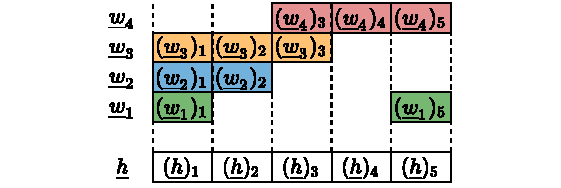
\includegraphics[trim={1.8cm 0 1.7cm 0},clip,scale=0.7]{images/parameter_mapping.pdf}}
    \subfloat[][]{\includestandalone[trim={0.65cm 0 0 0},clip,scale=0.7]{tikz/connection_matrix}}
    \subfloat[][]{\includestandalone[trim={0.6cm 0 0 0},clip,scale=0.6]{tikz/problem_splitting_matrix}}
    % \includestandalone[scale=1]{tikz/topology_general}
    \caption{Problem splitting and parameter mapping for a general case with \(M=5\) channels and \(P=4\) sub-problems. (a) shows the mapping of the local estimate components \((\wf_i)_j\) to the global consensus components \((\hf)_j\) via \(\mathcal{G}(i,j)\), (b) \(\mtxb{G}\) with 1 (\(\blacksquare\)) and 0 (\(\square\)), (c) shows \(i,j\)-cross-relations used by sub-problems compared to full \(M\)-channel problem.}
    \label{fig:problem_splitting:problem_splitting_matrix}
\end{figure}

% #############################################################################
\subsection{General Form Consensus ADMM}
\label{ssec:general_consensus_admm}
The separability of the problem can be used to take advantage of the well known alternating direction method of multipliers (ADMM).
Here more specifically, general form consensus ADMM \cite{}, which is used to minimize a problem of form
\begin{align}
    \operatorname{minimize} \quad &\sum_{i \in \Nset} \tilde{J}_i(\wf_i)\\
    \text{subject to} \quad &(\wf_i)_j = \hf_{\mathcal{G}(i,j)},\quad i \in \Nset,\,j \in \Cset_i
\end{align}
where \(\mathcal{G}(i,j)=g\) denotes the mapping of \(L\) local variable components \((\wf_i)_j\), i.e. one of the spectra in the stacked vector, to the corresponding global variable components \((\hf)_g\) (cf. \autoref{fig:problem_splitting:problem_splitting_matrix}). For brevity, a mapped global variable \(\tilde{\hf}_i\) with \((\tilde{\hf}_i)_j = \hf_{\mathcal{G}(i,j)}\) is defined.

The augmented Lagrangian for this particular general-form consensus problem is the real-valued function of a complex variable
\begin{align}
    &\mathcal{L}_{\rho} (\wf,\hf,\uuf) = \sum_{i \in \Mset} \left( \wf_i^\herm \aRhof_i \wf_i + \uuf_i^{\herm} \left(\wf_i - \tilde{\hf}_i\right)\vphantom{+ \frac{\rho}{2} \left\| \wf_i - \tilde{\hf}_i \right\|^2} \right.\nonumber\\
    &\left. + \left(\wf_i - \tilde{\hf}_i\right)^\herm \uuf_i + \left( \wf_i - \tilde{\hf}_i \right)^\herm \rho \I \left( \wf_i - \tilde{\hf}_i \right) \right).\label{eq:general_consensus_admm:lagrangian}
\end{align}
The ADMM then consists of the steps
\begin{align}
    &\wf_i^{k+1} = \underset{\wf_i}{\operatorname{argmin}} \left\{ \wf_i^\herm \aRhof_i \wf_i + \uuf_i^{k\,\herm} \left(\wf_i - \tilde{\hf}_i^{k}\right) \vphantom{+ \left\| \wf_i - \tilde{\hf}_i^{k} \right\|^2}\right.\nonumber\\
    &\left.+ \left(\wf_i - \tilde{\hf}_i^{k}\right)^\herm \uuf_i^{k} + \left( \wf_i - \tilde{\hf}_i^{k} \right)^\herm \rho \I \left( \wf_i - \tilde{\hf}_i^{k} \right) \right\}\label{eq:general_consensus_admm:local}\\
    &\hf^{k+1} = \underset{\hf, \|\hf\| = a}{\operatorname{argmin}} \left\{ \sum_{i \in \Mset} \left( \tilde{\hf}_i^{\herm} \uuf_i^{k} + \uuf_i^{k\,\herm} \tilde{\hf}_i \vphantom{\frac{\rho}{2} \| \wf_i^{k+1} - \tilde{\hf}_i \|^2} \right.\right.\nonumber\\
    &\left. \qquad \qquad \vphantom{\sum_{i=1}^{M} pp } \left.+ \left( \wf_i^{k+1} - \tilde{\hf}_i \right)^\herm \rho \I \left( \wf_i^{k+1} - \tilde{\hf}_i \right)  \right) \right\}\label{eq:general_consensus_admm:global}\\
    &\uuf_i^{k+1} = \uuf_i^{k} + \rho \left( \wf_i^{k+1} - \tilde{\hf}_i^{k+1} \right)\label{eq:general_consensus_admm:dual}
\end{align}

\subsection{Online ADMM}
\label{ssec:online_admm}
ADMM is originally an iterative method to solve optimization problems, however it has also been applied as an adaptive algorithm, also referred to as \emph{Online ADMM} \cite{}. The data term as part of \eqref{eq:general_consensus_admm:lagrangian} is time-dependent, which from here on will be denoted with the time index \(m\) in superscript \(\wf_i^\herm \aRhof_i^{m} \wf_i\).

The iterative form of the update steps as described in \eqref{eq:general_consensus_admm:local}-\eqref{eq:general_consensus_admm:dual} can be transformed into an adaptive one by computing a (small) finite number of iterations at each time step \(m\) with the current data term.
In this algorithm, one ADMM iteration is applied per time step, which simply allows us to replace the iteration index \(k\) with the time index \(m\).

The minimization problem \eqref{eq:general_consensus_admm:local} can be solved by various methods, in this case however we perform the update step
\begin{equation}
    \wf_i^{m+1} = \wf_i^{m} - \mu \bm{\mathcal{V}}_i^m \left( \aRhof_i^m \wf_i^m + \uuf_i^m + \rho\left(\wf_i^m - \tilde{\hf}_i^{m}\right)\right)\label{eq:online_admm:local_update}
\end{equation}
where \(0  < \mu\leq 1\) is a step size and \(\bm{\mathcal{V}}_i^m = \left(\aRhof_i^m + \rho \I \right)^{-1}\) is the inverse Hessian of the problem.
As this inverse is costly to compute, it is approximated by a diagonalized matrix
\begin{equation}
    \tilde{\bm{\mathcal{V}}}_i^m = \operatorname{diag} \left\{ \left( \operatorname{diag} \left\{ \aRhof_i^m \right\} + \rho \mtxb{1} \right)^{-1}\right\},
\end{equation}
similar to NMCFLMS \cite{}, which is straightforward to compute.

% To compute the consensus \(\hf\) we include the norm constraint \(\|\hf\| = a\) with a Lagrange multiplier \(\lambda\) in the minimization problem and replace the average of penalties with a penalty of averages which takes the form of
% \begin{attention}
%     poetic, cite our Boy[d]
% \end{attention}
% \begin{align}
%     \hf^{k+1} &= \underset{\hf}{\operatorname{argmin}} \left\{ \frac{\lambda}{2} \left(\hf^\herm \hf - a\right)\right.\nonumber\\
%     &\left. \qquad \qquad \quad + \frac{M \rho}{2} \left\| \hf - \bar{\wf}^{m+1} - \frac{1}{\rho} \bar{\uu}^{m} \right\|^2 \right\}\label{eq:online_admm:consensus_min_prob}
% \end{align}

For the consensus update step, it may be readily verified (cf. Boyd \cite{}) that the solution to \eqref{eq:general_consensus_admm:global} is given by
\begin{equation}
    \hf^{m+1} = a\frac{\bar{\wf}^{m+1} + \frac{1}{\rho} \bar{\uuf}^{m} }{\left\| \bar{\wf}^{m+1} + \frac{1}{\rho} \bar{\uuf}^{m} \right\|}.\label{eq:online_admm:consensus_update}
\end{equation}
where the \(M L \times 1\) vectors \(\bar{\wf}^{m+1}, \bar{\uuf}^{m+1}\) are computed as the mapped averages
\begin{equation}
    (\bar{\wf}^{m+1})_g = \frac{1}{N_g} \sum_{\mathcal{G}(i,j)=g} (\wf_i^{m+1})_j,\quad g,i,j \in \Mset,
\end{equation}
and
\begin{equation}
    (\bar{\uuf}^{m})_g = \frac{1}{N_g} \sum_{\mathcal{G}(i,j)=g} (\uuf_i^{m})_j,\quad g,i,j \in \Mset.
\end{equation}
This results in a computationally inexpensive update step forcing the norm of the consensus to have value \(a\).
% Algorithm \ref{alg:bsi_admm} summarizes the whole update procedure.
% \begin{attention}
%     Write down full algorithm
% \end{attention}

% \begin{algorithm}
%     \caption{BSI-ADMM}\label{alg:bsi_admm}
%     \begin{algorithmic}
%         \For {\(n=0,1,2,...\)}
%             \For{\(i \in \Mset\)}
%                 \State Acquire new data vector \(x_i^{(t)}\)
%                 \State Update \(\wf_i^{(n+1)} \leftarrow \wf_i^{(n)}\)
%             \EndFor
%             \State Update \(\hf^{(n+1)} \leftarrow \hf^{(n)}\)
%             \For{\(i \in \Mset\)}
%                 \State Update \(\uuf_i^{(t+1)} \leftarrow \uuf_i^{(n)}\)
%             \EndFor
%         \EndFor
%     \end{algorithmic}
% \end{algorithm}

% #############################################################################
% #############################################################################
\section{Numerical Evaluation}
\label{sec:perf_eval}

To asses the performance of the proposed algorithm and compare ot to state-of-the-art methods, numerical simulations are done.
The error measure to quantify system identification is the normalized projection misalignment (NPM) as used in other BSI-related literature \cite{}
\begin{equation}
    \text{NPM}(m) = 20\,\log_{10} \left(\frac{\left\| \h(m) - \frac{\h^\T (m) \h_{\text{t}}}{\h_{\text{t}}^\T \h_{\text{t}}}\h(m) \right\|_2}{\left\|\h(m)\right\|_2} \right)
\end{equation}
where \(\h\) is the stacked vector of impulse response estimates (cf. \autoref{ssec:cross_rel}), which are the inversely Fourier-transformed estimated spectra stacked in \(\hf\) and \(\h_{\text{t}}\) is the ground truth.

Similar to \cite{}, the first experiment aims to evaluate the performance of the algorithm on randomly generated impulse responses under different signal-to-noise ratios (SNR) using white Gaussian noise (WGN) as input signal and uncorrelated WGN independent between channels as additive noise.
The SNR is defined as
\begin{equation}
    \text{SNR} = 10 \log_{10} \left(\frac{\sigma_s^2 \| \h_t \|}{M \sigma_v^2} \right)
\end{equation}
where \(\sigma_s^2\) and \(\sigma_v^2\) are the variance of signal and noise respectively.

The impulse responses of length \(L=64\) are drawn from a Normal distribution with unit variance and the signal is 100 seconds of WGN to ensure convergence of all algorithms.
\autoref{fig:perf_eval:NPM_over_SNR} shows the median NPM of 30 Monte-Carlo runs where the averaged of the last \(100\) frames is taken as measurement.
\begin{attention}
    parameters
\end{attention}
It is observable that the proposed algorithm yields a lower steady-state NPM than the compared NMCFLMS, RNMCFLMS, and \(l_p\)-RNMCFLMS algorithms.
\begin{figure}
    \centering
    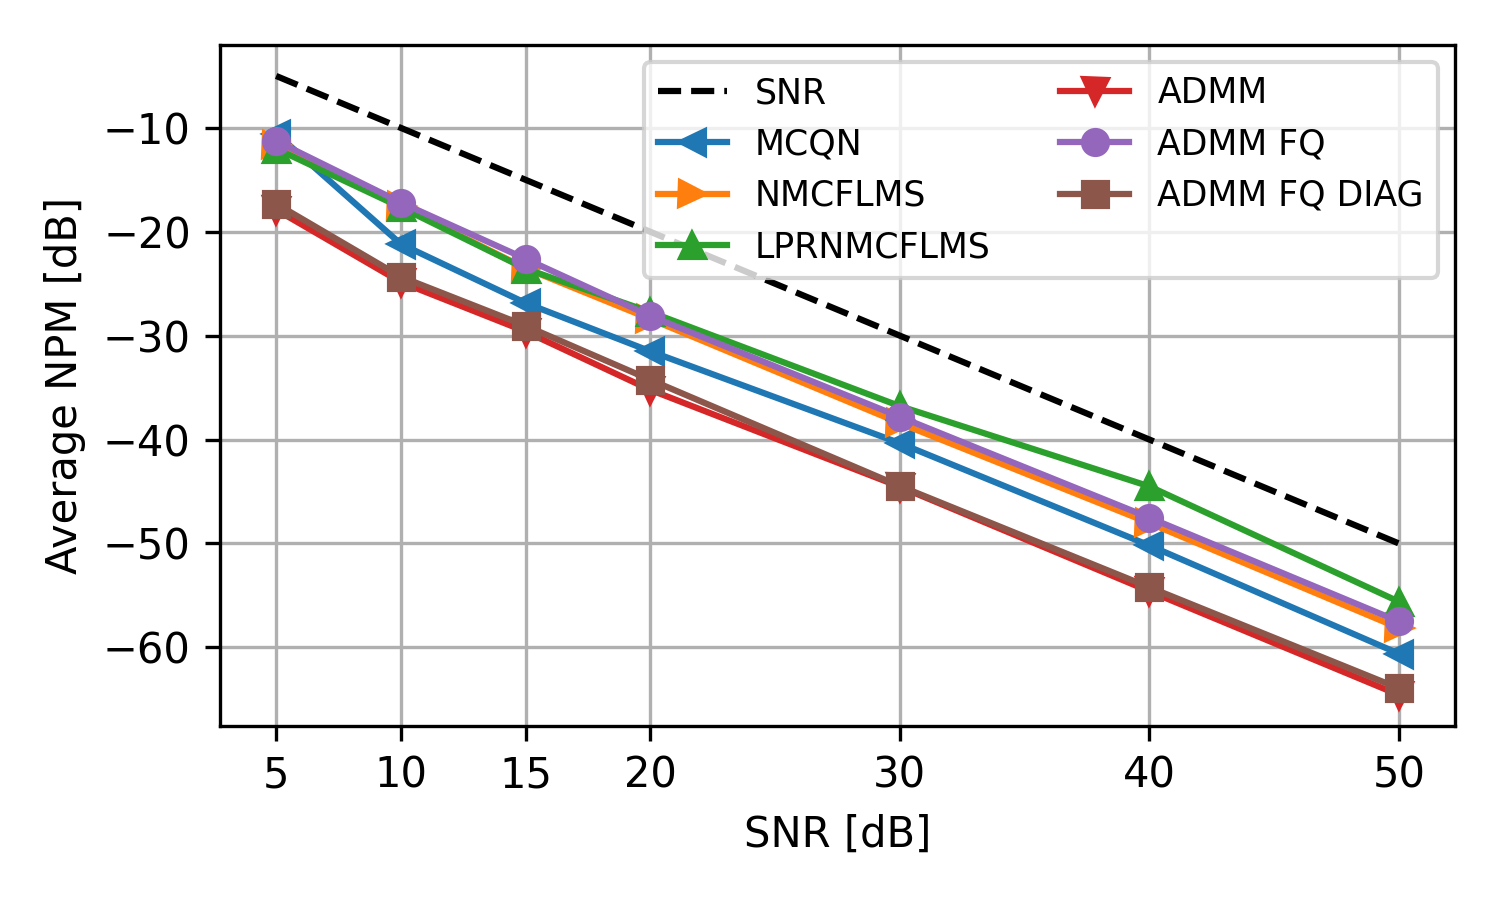
\includegraphics[height=5cm]{python/plots/NPM_over_SNR_L16.png}
    \caption{Steady-state NPM of ADMM-BSI and compared algorithms over different SNRs.}
    \label{fig:perf_eval:NPM_over_SNR}
\end{figure}

The second experiment is a small scale assessment of the influence of the overlap of sub-problems.
Two base scenarios, \(M=4,P=4\) and \(M=8,P=8\), are evaluated using short (\(L=16\)) random impulse responses and different values for the sub-problem overlap parameter \(\zeta\) which is defined as the ratio of ones to zeros of only considering elements of \(\mtxb{G}\) that are not part of the main diagonal, superdiagonal and the first element of the last row (marked gray in \autoref{fig:perf_eval:NPM_over_time_M4}).
Random patterns satisfying this definition for \(\zeta \in \{0.0,\,0.25,\,0.5,\,0.75\}\) and random impulse responses with \(L=16\) are generated and the algorithm is applied.
\autoref{fig:perf_eval:NPM_over_time} shows the median of 30 Monte-Carlo runs for the two setups, which lets us observe the proportional relation of convergence speed, channel number \(M\) and sub-problem overlap \(\zeta\).
Note that the steady state error is not dependent on \(\zeta\).
\begin{attention}
    parameters
\end{attention}

\begin{figure}
    \centering
    % \hspace*{-0.4cm}\subfloat[][\(M\!=\!4,P\!=\!4\)]{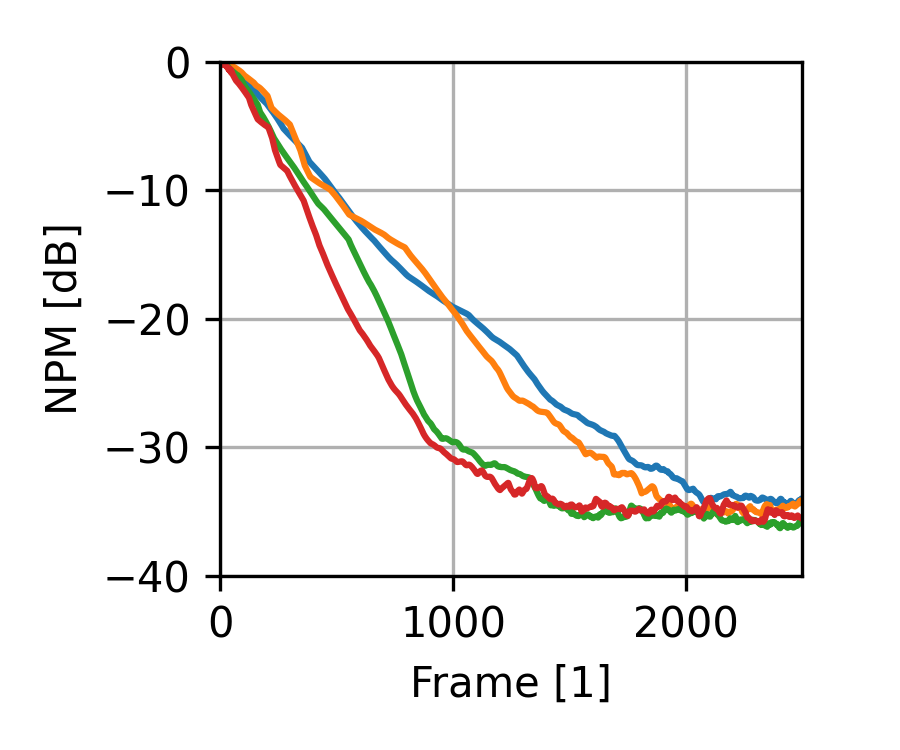
\includegraphics[height=4cm]{python/plots/NPM_over_time_M4.png}\label{fig:perf_eval:NPM_over_time_M4}}
    \hspace*{-0.4cm}\subfloat[][\(M\!=\!4,P\!=\!4\)]{\begin{overpic}[height=4cm]{python/plots/NPM_over_time_M4.png}
        \put(54,48){\includestandalone[scale=0.5]{tikz/connection_matrix_eval}}
    \end{overpic}\label{fig:perf_eval:NPM_over_time_M4}}
    \hspace*{-0.5cm}\subfloat[][\(M\!=\!8,P\!=\!8\)]{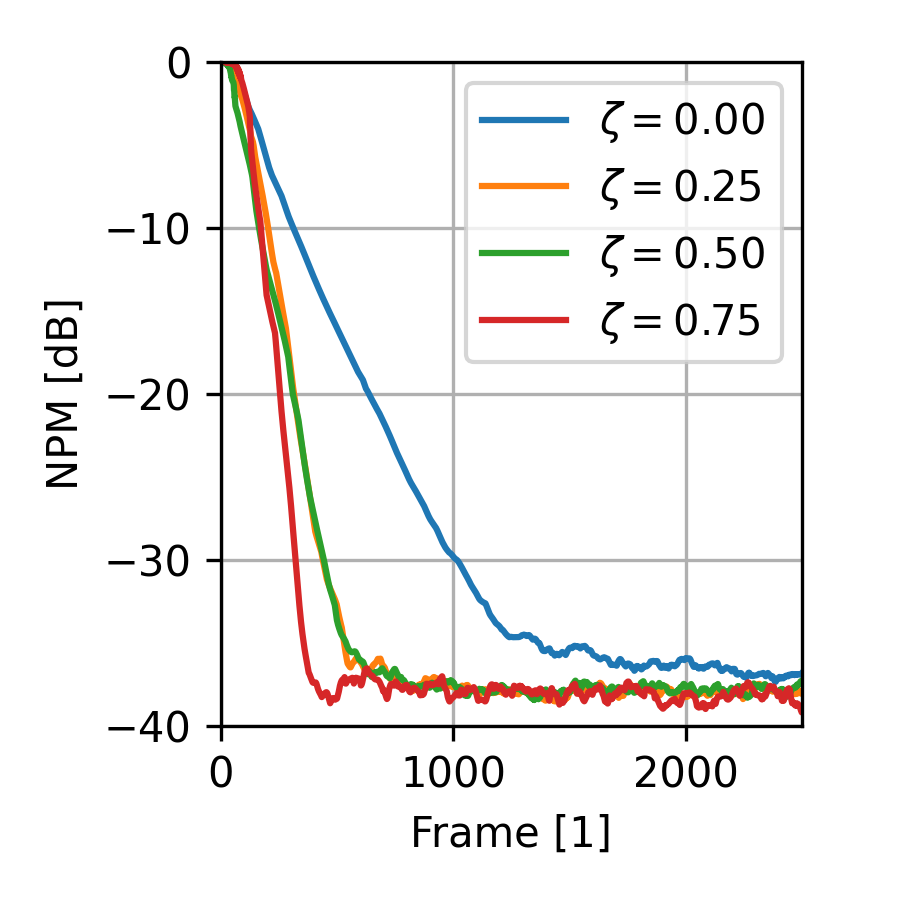
\includegraphics[height=4cm]{python/plots/NPM_over_time_M8.png}\label{fig:perf_eval:NPM_over_time_M8}}
    \caption{Comparison of ADMM-BSI convergence behaviour with \(L\!=\!16\) for different values of the sub-problem overlap \(\zeta\).}
    \label{fig:perf_eval:NPM_over_time}
\end{figure}

\begin{attention}
    Or if figured out, do longer simulated acoustic impulse responses.
\end{attention}


% #############################################################################
% #############################################################################
\section{Conclusions}
\label{sec:conclusion}
In this paper, an adaptive ADMM algorithm for blind system identification was introduced.
The algorithm splits the BSI problem into lower-dimensional sub-problems to reduce complexity and allow parallel processing.
The the identification performance of the algorithm is compared to state-of-the-art algorithms and shows improved steady-state error measures.

% References should be produced using the bibtex program from suitable
% BiBTeX files (here: strings, refs, manuals). The IEEEbib.bst bibliography
% style file from IEEE produces unsorted bibliography list.
% -------------------------------------------------------------------------
% \bibliographystyle{IEEEbib}
% \bibliography{refs}

\end{document}